\section{\concept{} Overview} \label{sec:system}
In this section, we first give the programming model of \concept{}, followed by
its architecture, and the workflow to transform a high-level SDC program to
datapath configurations with local state sharing.

%including the translation from programs into flow rules at switches and configurations of middleboxes (\ie, how to interact with switches). We will start with the extension of programming model from SNAP (XXX) and then describe each component of the system.

\vspace{-2mm}
\subsection{Programming Model}
\concept{} adopts an omnipotent programming model proposed in high-level SDN
programming systems (\eg, Maple~\cite{maple}), which logically programs every single packet with an
onPacket function. In addition to the primitives that read and test on packet
headers, \concept{} designs the following primitives for users to model and
specify middleboxes in SDC network. The first is to specify a middlebox in the network (\codeword{m = middlebox(name,
property)}) where the property indicates the middlebox is stateless or not; The
second is to
invoke the packet handling of a middlebox (\codeword{m.handle(pkt)}).
Specifically, we consider a middlebox as a packet handling function that can
return the result for the incoming packet. For the stateless middlebox, if two
packets have the same 5-tuple match fields, they always have the same
results. For the stateful middlebox, this cannot be guaranteed as the packet
processing depends on the state in the middlebox.

%To handle the returned result of a middlebox for a packet, we consider the
%following switch-middlebox interaction process. 
In \concept{}, the interaction between switch and middlebox is bi-directional.
A switch can send a packet to a
middlebox for the processing through a tunnel. After the processing, the middlebox can send
the packet back and share its local state of the packet %(5-tuple flow matches)
with switches. In \concept{}, such interaction is transparent to the user so that
the user does not need to manually configure the local state sharing between
data plane devices. Instead, as we will show in the next section, \concept{}
automatically translates high-level SDC programs into data plane configurations
with local state sharing.

%To reUser is unaware of such interaction. Instead,

%is transparent to the user. 
%(leveraging their stateful datapath design). %Note that by using
%tunnels, any switch can send a packet to any middlebox, and also the inverse.

%Though the interaction is simple, there are several details need to consider
%(\eg, in the step 3 of the \concept{} design for the firewall example, how to
%guarantee that the packet gets the newest state?). We will talk about the
%details in the next section.

In addition to the middlebox primitives, \concept{} also adopts the route algebra
primitive~\cite{gao2018t} for the user to specify path constraints for packets
forwarding in SDC network. The abstract syntax of the \concept{} programming model
is shown in Fig~\ref{fig:grammar1}. Specifically, for the route algebra expressions, we adopt the same in~\cite{gao2018t}. For the middlebox, programmers can specify its property, \ie, stateless or stateful. 
%Inside the onPacket program, besides the basic packet test statements, programmers can specify a middlebox operation to handle packets. Also the route algebra variable should be the return as it gives the path constraints.

%Therefore, we consider the three kinds of statements
%(besides the basic control statements such as \codeword{if, else}): 1. Test of
%packet match fields; 2. Packet handling of a middlebox; 3. Route algebra as a
%return.

\begin{figure}[ht]
{%\small
% \fontsize{10}{12}\selectfont 
\scriptsize
%{\bf Abstract syntax:}
%\vspace{-2mm}
\[%\arraycolsep=1.4pt\def\arraystretch{2.2}
\begin{array}{rclr}
p &\bnfdef & \ONPKT\ \{I\},\ d_1,\ \ldots,\ d_n &(\textit{program})\\
d &\bnfdef & x^r\ =\ r\  & (\textit{route algebra decl})\\
 & & \bnfalt x^m\ =\ middlebox(n,\ s) & (\textit{middlebox decl})\\
I &\bnfdef & x\ =\ e & \\
 & & \bnfalt I;I &  (\textit{sequencing})\\
 & & \bnfalt x\ =\ x^m.handle(pkt) &  (\textit{middlebox operation})\\
 & & \bnfalt \ifelse{e^b}{I}{I} &  (\textit{conditional})\\ %\\ 
 & & \bnfalt \return{x^r} \bnfalt \return{r} &  (\textit{func return})\\ 
% & & \bnfalt m[e_1, \dots, e_n] := e & (\textit{map update}) \\
% & & \bnfalt s := s \cup \{e\} \bnfalt s := s - \{e\} & (\textit{set update}) \\
e &\bnfdef & c \bnfalt x &  (\textit{consts, vars})\\
%& & \bnfalt x^r  & (\textit{route algebra vars}) \\
& & \bnfalt x^m & (\textit{middlebox vars}) \\
& & \bnfalt pkt.a & (\textit{packet fields}) \\
% & & \bnfalt e+e \bnfalt e*e \dots & (\textit{arith}) \\ 
e^r & \bnfdef & e == e \bnfalt e \leq e \dots & (\textit{relational})\\
e^b & \bnfdef & e^r \bnfalt e^r\ \&\ e^r \bnfalt e^r\ |\ e^r \dots & (\textit{boolean})\\
(r &{\color{blue}{\in}}&\mathit{route\ algebra\ expressions}) & \\
(c &{\color{blue}{\in}}& \mathit{strings}) & (\mathit{consts})\\
(a &{\color{blue}{\in}}& \{ \mathit{macSrc}, \mathit{ipDst} \dots \}) & (\textit{packet fields})\\
(n &{\color{blue}{\in}}& \mathit{strings})  &  (\textit{middlebox names})\\
(s &{\color{blue}{\in}}& \{ \mathit{stateless},\mathit{stateful} \})  &  (\textit{properties})\\
(x &{\color{blue}{\in}} & \{\tx_1,\tx_2,\dots,\ty_1,\dots\}) &  (\textit{variables})\\
\end{array}\]}% small
%\vspace{1mm}
% \hrule
%\vspace{-5mm}
\caption{\concept{} abstract syntax.}
\label{fig:grammar1}
\end{figure}



\para{Example \concept{} program:} Revisit the motivating example in Section~\ref{sec:motivation}, the network
operator can specify the policy to forward packets of sensitive and non-sensitive data along different paths using the \concept{} program in Fig.~\ref{fig:code}.
%to forward packets of sensitive and non-sensitive data along different paths using the \concept{} program in Fig.~\ref{fig:code}.

\begin{figure}[h]
\begin{scriptsize}
\begin{verbatim}
L1: mFW = middlebox("firewall", "stateless")
L2: PATH1 = h1 -> b -> h2 //b: waypoint
L3: PATH2 = h1 -> c -> h2 //c: waypoint
L4: //any: picking any path
L5: def onPacket(pkt):
L6:   if pkt.srcAddr == h1 & pkt.dsrAddr == h2:
L7:     if mFW.handle(pkt) == SENSITIVE:
L8:       return any(SPC.stable + PATH1)
L9:     else:
L10:      return any(SPC.stable + PATH2)
L11:  else: return DROP
\end{verbatim}
\end{scriptsize}
	\caption{\small The \concept{} program for the policy in the motivating example. For line 8 (9), the correct versions are in their comments.}
\label{fig:code}
\end{figure}

Specifically, line 2 (3) specifies a path constraint that starts from $h_1$ to $h_2$ and must pass through $b$ ($c$) (Note that it does not represent a concrete path but a path constraint). And the return statements use \emph{any} function (defined in route algebra~\cite{gao2018t}) that picks any path satisfying the constraint. Although the programming model is quite simple, as involving middleboxes which physically map to nodes in the network, the system needs to guarantee the correctness for the program.

\para{Correctness}: We denote the correctness as the following: For any packet $pkt$, the real forwarding path for $pkt$ in the network must comply with the returned path for $pkt$ in the program. For example, if the programmer uses \emph{opt} function to pick the shortest hop count path with the constraint (\ie, \codeword{opt(PATH1)}), then the returned path is $gw, a, b, d$. However, as the (first) packet must access the firewall, the real path must include $fw$ which does not comply with the returned path in the program.

One simple solution to guarantee the correctness is to let the programmer explicitly include the necessary middlebox nodes in the path constraint. In this case, it should be \codeword{PATH1 = h1 -> fw -> b -> h2}. However, this can add extra burden to programmers that they should make sure the path constraints comply with the traces of packets in the network.

\para{System Path Constraint}: To resolve the issue, we introduce the System Path Constraint (SPC) which is a global variable storing path constraints that must be complied with when computing a path at any location in the program. The intuition is that when a packet going through the program, some statements can add path constraints for the packet. For example, in Fig.~\ref{fig:code}, line 6 adds a constraint that the path should start from $h_1$ to $h_2$; Line 7 adds a constraint that the path must include the firewall. Then, after line 7, the SPC variable includes constraints that the path starts from $h_1$ to $h_2$ and includes $fw$. If the line 8 uses the \emph{opt} function, then it should be \codeword{return opt(SPC + PATH1)} where the ``+'' means connecting the waypoints constraints in SPC and PATH1, and its result is $gw, fw, a, b, d$. (Note that the definition of \codeword{SPC.stable} will be given in the next section.)

%And the programmer should include the SPC variable when computing the path in line 8 (\ie, \codeword{return any(SPC + PATH1)} where the ``+'' means connecting the waypoints constraints in SPC and PATH1). As such, the result of \codeword{opt(SPC + PATH1)} should be $gw, fw, a, b, d$.

%
%\begin{figure}[h]
%\begin{footnotesize}
%\begin{verbatim}
%L1: mFW = middlebox("firewall")
%L2: PATH1 = h1 -> mFW -> b -> h2 //b: waypoint
%L3: PATH2 = h1 -> mFW -> c -> h2 //c: waypoint
%L4: opt := picking shortest hop count path
%L5: def onPacket(pkt):
%L6:     if pkt.srcAddr == h1 & pkt.dsrAddr == h2:
%L7:         if mFW.handle(pkt) == SENSITIVE:
%L8:             return opt(PATH1) 
%L9:         else:
%L10:           return opt(PATH2)
%L11:    else: return DROP
%\end{verbatim}
%\end{footnotesize}
%	\caption{\small The \concept{} program for the policy in the motivating example.}
%\label{fig:code}
%\end{figure}
%
%\begin{figure}[h]
%\begin{footnotesize}
%\begin{verbatim}
%L1: mFW = middlebox("firewall")
%L2: PATH1 = h1 -> b -> h2 //b: waypoint
%L3: PATH2 = h1 -> c -> h2 //c: waypoint
%L4: opt := picking shortest hop count path
%L5: def onPacket(pkt):
%L6:     if pkt.srcAddr == h1 & pkt.dsrAddr == h2:
%L7:         if mFW.handle(pkt) == SENSITIVE:
%L8:             return opt(SPC.stable + PATH1) 
%L9:         else:
%L10:           return opt(SPC.stable + PATH2)
%L11:    else: return DROP
%\end{verbatim}
%\end{footnotesize}
%	\caption{\small The \concept{} program for the policy in the motivating example.}
%\label{fig:code}
%\end{figure}

%Since we do not focus on the state operation deployment (which is the major component of SNAP), we only considers two kinds of statements that can apply to packets: 1. Test of packet match fields (\eg, line 6 in the firewall program); 2. Packet handling of middlebox (\eg, line 7 in the firewall program). The former one is the same with the SNAP and the latter one returns the result of packet handling of a middlebox.

%
%Also, as only stateless middleboxes can leverage stateful switches as the cache of results of its packet processing, the system needs to identify whether a middlebox is stateless or not. For simplicity, we make the programmer give the hint. In the program, when initializing a middlebox variable, the program should specify whether it is stateless or not. The following gives an example that how to give a hint at the middlebox variable initializing statement.
%
%\begin{small}
%\begin{verbatim}
%mFW = middlebox("firewall", "stateless")
%...
%if mFW.handle(pkt) = GOOD:
%\end{verbatim}
%\end{small}
%
%
%\subsection{Middlebox Behavior}
%
%We consider a middlebox as a packet handling function that can return the result for the incoming packet. For the stateless middlebox, if two packets have the same 5-tuple match fields, then they always have the same results. For the stateful middlebox, this cannot be guaranteed as its packet processing depends on the state in the middlebox.
%
%For the interaction between a middlebox and a switch, we consider the following model. A switch can send a packet to a middlebox for the processing, and after the processing the middlebox can send the packet back and update a flow's state (based on the result) at any switch. (The flow has the same 5-tuple with the packet.) This process is very similar with the interaction between OpenFlow switches and the controller which includes packet-in message, packet-out message, and OpenFlow rules update. Note that by using tunnels, any switch can send a packet to any middlebox, and also the inverse. Though the interaction is simple, there are several details need to consider (\eg, in the step 3 of the \concept{} design for the firewall example, how to guarantee that the packet gets the newest state?). We will talk about the details in the next section.

\vspace{-2mm}
\subsection{Architecture and Workflow}
Fig.~\ref{fig:system-workflow} presents the architecture and workflow on how
\concept{} translates high-level \concept{} SDC programs to low-level
configurations of data plane devices with local state sharing. Given a
high-level \concept{} SDC program, \concept{} first computes a decision graph that captures the forwarding decisions process of
packets and stateful operations on packets. Second, \concept{} computes optimal
paths for packet forwarding in the network with a system defined objective (\eg,
maximizing total throughput). \textbf{Note} that the system computes paths when the returned paths are not concrete (\eg, using $any$ function), and in the remaining part of the paper, we assume these paths are not concrete to introduce the path computation part. Third, the device-level data plane configurations are generated, which
include local state sharing configurations, so that devices can exchange local
state to forward the packets along the computed optimal paths. \concept{} leverages the stateful switch for local state sharing which includes two match-action tables: one is
a state table (\ie, $match \rightarrow state$) and the other is a match table
(\ie, $match+state \rightarrow action$). Given a switch, a
packet first enters the state table to get its corresponding state (by matching
its packet fields) and then enters the match table to get the action.

%from the program (and the definition of DG
%will be shown in the next section). Step 2: Based on the DG and the topology,
%Step 3: Generate datapath configuration in the network.

\begin{figure}[!htbp]
%\vspace{-2mm}
\centering
\begin{subfigure}{0.4\linewidth}
      \centering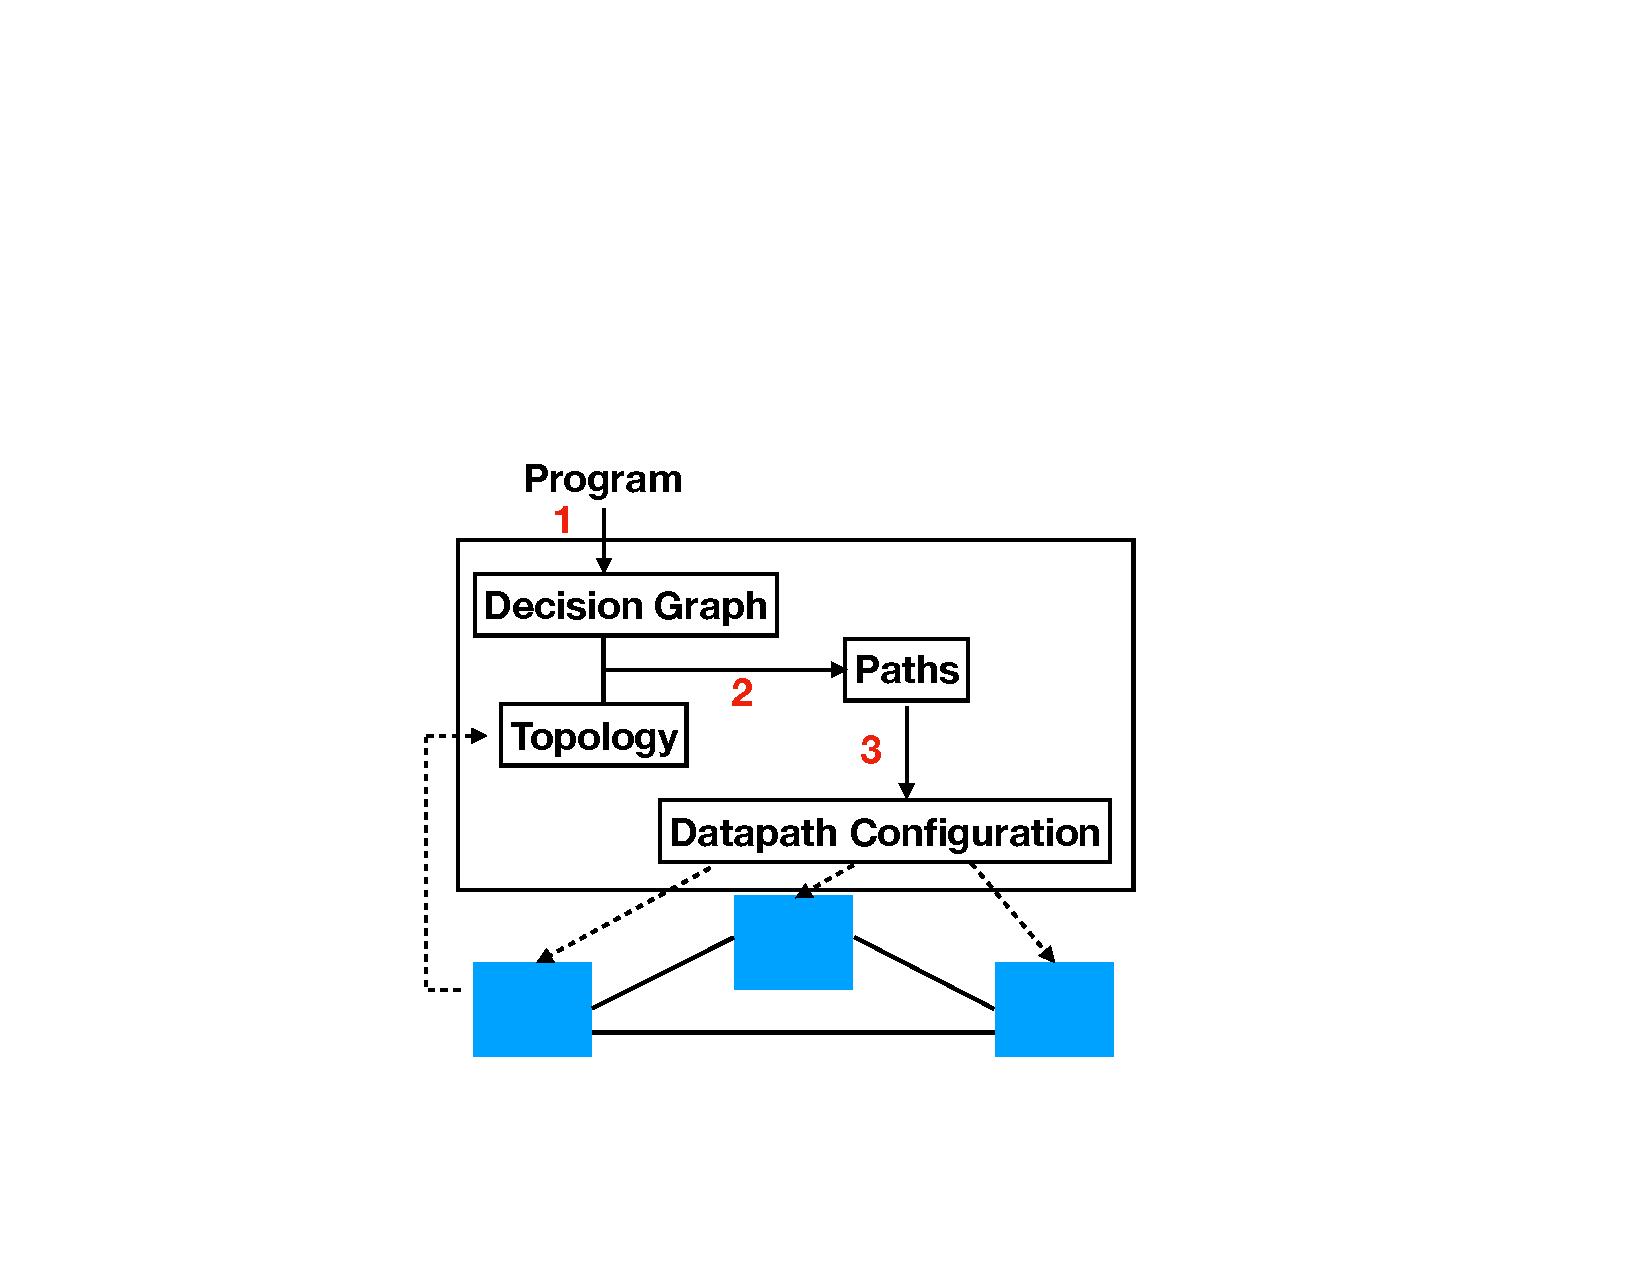
\includegraphics[width=\linewidth]{figures/ss-125.pdf}
\end{subfigure}
%\vspace{-2mm}
%\caption{\footnotesize{The CDF of job latency local and remote jobs.}}
\caption{\small The architecture and workflow of \concept{}.}
%\vspace{-2mm}
\label{fig:system-workflow}
\end{figure}

\begin{figure}[!htbp]
%\vspace{-2mm}
\centering
      \centering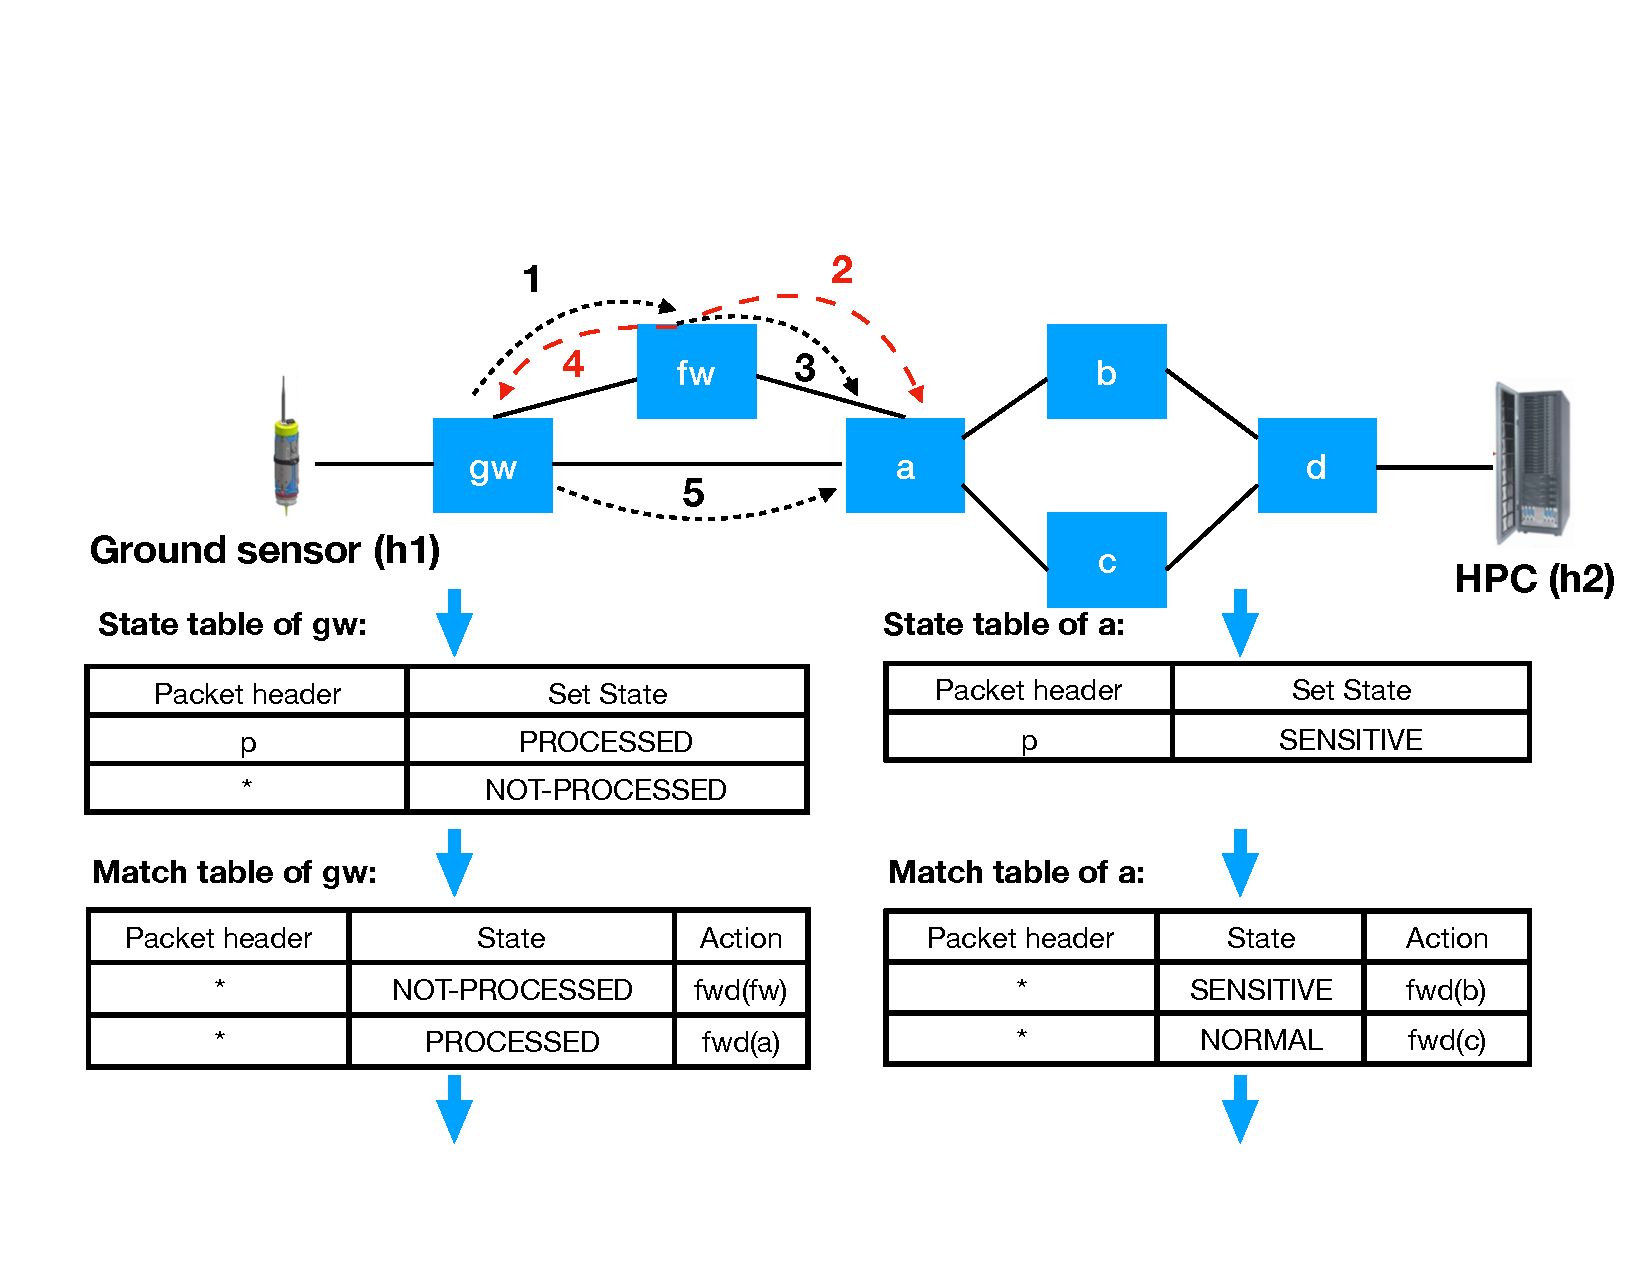
\includegraphics[width=0.8\linewidth]{figures/ss-124.pdf}
   %\vspace{-2mm}
%\caption{\footnotesize{The CDF of job latency local and remote jobs.}}
	\caption{\small The configuration translated by \concept{} from the
	program in Fig.~\ref{fig:code}.}
%\vspace{-2mm}
\label{fig:dsdc-result}
\end{figure}

\para{Example configuration with local state sharing}:  
Fig.~\ref{fig:dsdc-result} gives the data plane configuration with local state
sharing translated from the SDC program in Fig.~\ref{fig:code}. Specifically,
by allowing the local state sharing, the
firewall $fw$ can share its local identification state for a flow with the
gateway switch $gw$.
For example, it can send the state: 
$srcAddr=h1,dstAddr=h2,srcPort=12345,dstPort=22,protocol=tcp \rightarrow$
\emph{PROCESSED} to $gw$, which can insert it into its state table.

With this configuration, the first packet $p$ arrives at the
gateway $gw$ is forwarded to $fw$ by getting a state
\emph{NOT-PROCESSED} at $gw$ (Step 1). Assume $fw$ identifies $p$ as \emph{SENSITIVE}.
It first sends this local state $p \rightarrow SENSITIVE$ to $a$ (Step 2). Next,  $fw$
forwards $p$ to $a$ (Step 3), where $p$ is forwarded to $b$ because its state is \emph{SENSITIVE}. 
Then $fw$ sends the local state $p \rightarrow PROCESSED$ to $gw$ (Step 4). As such, all future packets with the
same match fields as $p$ entering $gw$ will be forwarded directly to $a$ (Step 5).

%design which leverages this local state
%sharing. We assume 



%The design with \concept{} has 5 steps: 

 



%
%In this section, we will first give basic concepts and the target for general network-wide stateful packet processing in data planes. Then, the consistency requirement will be discussed based on the basic concepts.
%
%\subsection{basic concepts and the target}
%
%\para{State variable and operations}: State variables are the persistent states on the data planes (stateful switches). In this paper, for the simplicity, we consider the state variable as a key-value map whose key can be matched by the fields of packets. For the read operation of state variables, an incoming packet ($pkt$) can read a value of an entry in the map ($m$) and store the value to the packet's meta data [ref: meta data XXX] by matching the fields ($f$) of the packet (note that the fields include meta data); for the write operation, flow tables can support a special state-update action that can update the map (including modify the value of a specific entry in the map and/or add a new entry to the map). 
%
%%The formal expressions of the two operations are shown in the Figure 2 XXX.
%
%%Figure formal expression.
%
%\para{General network-wide stateful packet processing}: Network-wide stateful packet processing for a packet can be viewed as a sequence of read/write operations of the state variables applied by the packet. Given a state variable (map) $m_k$, we denote $o_i^{s(i)}$ as the operation with $m_k$ indicated by $s(i) = k$. Then, we have a sequence of $n$ operations (denoted as $O$) as $o_1^{s(1)}, o_2^{s(2)}, ..., o_i^{s(i)}, ..., o_n^{s(n)}$. 
%We denote a sequence of operations $O$ with at most two operations $o_i^{s(i)}, o_j^{s(j)}$ in $O$ that they have $s(i) = s(j) = k$ and $i \neq j$ as \emph{one-loop} sequence for $m_k$ and $o_i^{s(i)}, o_j^{s(j)}$ as its \emph{end-loop} operations.
%For the existing work (\ie, SNAP), for any \emph{one-loop} sequence, all the state variables (\ie, maps) involved in the sequence between its \emph{end-loop} operations (including \emph{end-loop} operations) should be stored in a \textbf{single} switch. 
%This is why it cannot achieve the load-balancing example in Sec. 1. 
%
%\para{Target}: For the proposed \textbf{general} network-wide stateful packet processing, we relax the constraint of single switch and our target is to support a more flexible sequence of read/write operations with less constraints for putting which state variables to which switches. (Note that a state variable should be placed on a single stateful switch.) Specifically, given a state variable $m_k$ and a flow with requirements to access $m_k$, the flow can apply at most one \emph{one-loop} sequence for $m_k$ where the state variables involved in the operations between its \emph{end-loop} operations can be spread to \textbf{multiple} switches. For the example in Figure 2, state variable $m_k$ is $sw_1$ and two flows $flow_1$ and $flow_2$ access $m_k$. Flow $flow_1$ has two sequences of operations: $op_{11}, op_{12}, op_{13}$ and $op_{11}, op_{12}, op_{14}, op_{15}$. Both sequences are \emph{one-loop} sequences for $m_k$ as all $op_{11}, op_{13}, op_{15}$ involve $m_k$. Then, this is not supported in our target. If $flow_1$ only keeps $op_{11}, op_{12}, op_{13}$, then the sequence of operations of $flow_2$ also can be supported.
%
%However, this flexibility may arise consistency issue which will be discussed in the following subsection.
%
%\begin{figure}[!htbp]
%%\vspace{-2mm}
%\centering
%\begin{subfigure}{0.7\linewidth}
%      \centering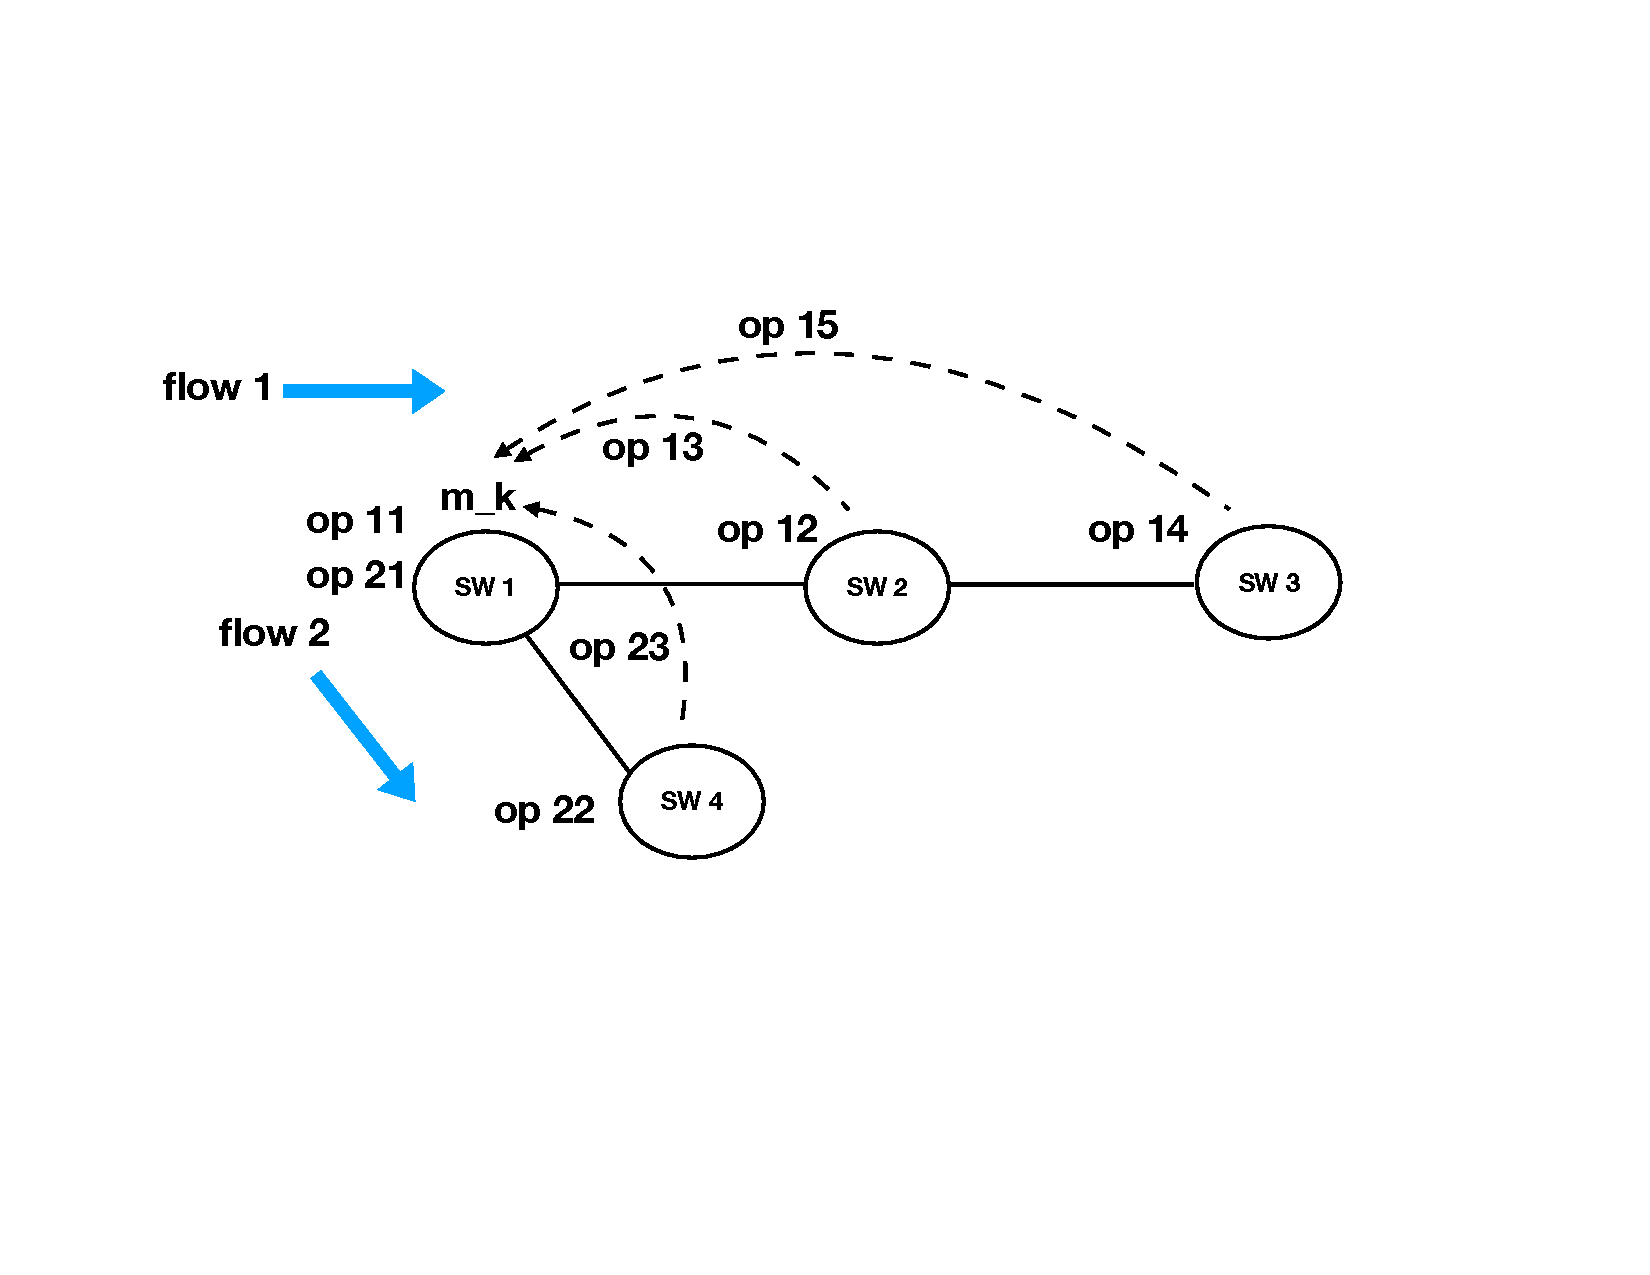
\includegraphics[width=\linewidth]{figures/68.pdf}
%\end{subfigure}
%%\vspace{-2mm}
%%\caption{\footnotesize{The CDF of job latency local and remote jobs.}}
%\caption{\small Example of \emph{one-loop} sequence.}
%%\vspace{-2mm}
%\label{fig:mtv-example}
%\end{figure}
%
%\subsection{consistency requirement}
%
%%As a flow consists of a sequence of packets, for any event caused by a packet, the event should be noticed by the following packets in the flow. In the stateful packet processing setting, we should have the following consistency requirement. 
%
%First, consistency should be considered when a packet $pkt_i$ (belonging to a flow with a sequence of packets $pkt_1, pkt_2, ..., pkt_i, ...$ where a packet with a smaller index appears at the network earlier) tries to access a state variable $m_k$. We denote the sequence of historical state operations of $pkt_i$ as $HO(pkt_i)$. Also, we have a sequence of packets $pkt_{i1}, pkt_{i2}, ..., pkt_{ih}$ (denoted as $D(pkt_i)$) as a subsequence of $pkt_1, pkt_2, ..., pkt_{i-1}$ that $\forall pkt_{ij} in D(pkt_i), HO(pkt_i) is the prefix of HO(pkt_{ij})$. Then, the consistency requirement is that $\forall pkt_{ij} \in D(pkt_i)$, for the value of $m_k$ updated by $pkt_{ij}$, $pkt_i$ must see the updated value of $m_k$. In other words, if $pkt_{i-1}$ and $pkt_i$ following the same path with the same state operations to a stateful switch $sw$, $pkt_i$ (and the following packets) must see any update to any state variables at $sw$ as long as these updates comes from $pkt_{i-1}$. If two packets do not have the same historical state operations, as the order of the two packets itself cannot guarantee, the consistency also should not be considered.
%
%%Given a flow with a sequence of packets $pkt_1, pkt_2, ..., pkt_i, ...$ (a packet with a smaller index appears at the network earlier) and a set of state variables (maps) $M$, we denote the value of $M$ as $M_i$ if it is just before $pkt_i$ is processed by a sequence of state operations with $M$ and $M_i'$ if it is just after $pkt_i$ is processed. Then, the consistency requirement is: $\forall pkt_i, M_i = M_{i-1}'$ ($M_0$ means the original states). In other words, if $pkt_i$ updates any states, $pkt_{i+1}$ (and the following packets) should see the updated states.
%
%In a simple SDN network, the consistency requirement is easy to guarantee as all the states are in the logical centralized controller. Also, the consistency in the single switch design for \emph{one-loop} sequences is also easy to achieve as a single switch can store complex data dependency among state variables.
%%given a sequence of state operations $O$, if there are any two operations with the same state variable in $O$ and all the state variables between these two operations are placed in a single switch
%%the consistency is also easy to guarantee if all the state variables between these two operations are placed in a single switch. 
%However, in the proposed general network-wide stateful packet processing, it is not easy to guarantee as a packet can jump to the previous switch to update a state variable that has been updated before by the packet. We will discuss how the consistency guaranteed in the following section.
%




